\chapter{Theory}
\label{cha:theory}

% ~10p

% The main purpose of this chapter is to make it obvious for
% the reader that the report authors have made an effort to read
% up on related research and other information of relevance for
% the research questions. It is a question of trust. Can I as a
% reader rely on what the authors are saying? If it is obvious
% that the authors know the topic area well and clearly present
% their lessons learned, it raises the perceived quality of the
% entire report.
% 
% After having read the theory chapter it shall be obvious for          <--
% the reader that the research questions are both well                  <--
% formulated and relevant.                                              <--
% 
% The chapter must contain theory of use for the intended
% study, both in terms of technique and method. If a final thesis
% project is about the development of a new search engine for
% a certain application domain, the theory must bring up related
% work on search algorithms and related techniques, but also
% methods for evaluating search engines, including
% performance measures such as precision, accuracy and
% recall.
% 
% The chapter shall be structured thematically, not per author.
% A good approach to making a review of scientific literature
% is to use \emph{Google Scholar} (which also has the useful function
% \emph{Cite}). By iterating between searching for articles and reading
% abstracts to find new terms to guide further searches, it is
% fairly straight forward to locate good and relevant
% information, such as \cite{test}.
% 
% Having found a relevant article one can use the function for
% viewing other articles that have cited this particular article,
% and also go through the article’s own reference list. Among
% these articles on can often find other interesting articles and
% thus proceed further.
% 
% It can also be a good idea to consider which sources seem
% most relevant for the problem area at hand. Are there any
% special conference or journal that often occurs one can search
% in more detail in lists of published articles from these venues
% in particular. One can also search for the web sites of
% important authors and investigate what they have published
% in general.
% 
% This chapter is called either \emph{Theory, Related Work}, or
% \emph{Related Research}. Check with your supervisor.

This chapter introduces background and related work.

% background: neuroscience, framework
% related work: practical aspects, reinforcement learning

\section{Background}

\subsection{Active Vision}

% Marr?

Much of past and present research in machine perception involves a passive observer.
Images are passively sampled and perceived.
Animal perception, however, is active.
We do not only see things, but look for them.
One might ask why this is the case, if there is any advantage that an active observer has over a passive one.
Aloimonos and Weiss (1988)~\cite{aloimonos_active_1988} introduce the paradigm called \textit{active vision}, and prove that an active observer can solve several basic vision problems in a more efficient way than a passive one.

Bajcsy (1988)~\cite{bajcsy_1988} defines active vision, and perception in general, as a problem of intelligent data acquisition.
An active observer needs to define and measure parameters and errors from its scene and feed then back to control the data acquisition process.
Bajscy states that one of the difficulties of this problem is that they are scene and context dependent.
A thorough understanding of the data acquisition parameters and the goal of the visual processing is needed.
One view lacks information that may be present with multiple views.
Multiple views also add the time dimension into the problem.

In a re-visitation of active perception, Bajcsy, Aloimonos and Tsotsos (2018)~\cite{bajcsy_aloimonos_tsotsos_2018} stress that despite recent successes in robotics, artificial intelligence and computer vision, an intelligent agent must include active perception:

\begin{quote}
    An agent is an active perceiver if it knows why it wishes to sense, and then chooses what to perceive, and determines how, when and where to achieve that perception
\end{quote}~\cite{bajcsy_aloimonos_tsotsos_2018}

% see conclusion in that paper:
% - mirror neurons, same system responsible for generating and interpreting actions at a high level 

\cite{chen_activevisionsurvey_2011}

\subsection{Visual Search}
\label{sec:visualsearch}

% todo: should maybe remove the psychology and keep that in introduction only
% "kuriosa"

The perceptual task of searching for something in a visual environment is usually referred to as \textit{visual search}.
The searched object or feature is the \textit{target}, and the other objects or features in the environment are the \textit{distractors}.
This task has been studied extensively in psychology and neuroscience.
% the reason for introducing this is to be able to use the same terminology later

Wolfe (2021)~\cite{wolfe_guided_2021} describes a model of visual search

% general things
% - foveated vision
% - covert and overt attention

Eckstein (2011)~\cite{eckstein_visual_2011} reviews efforts from various subfields and identifies a set of mechanisms used to achieve efficient visual search.
Knowledge about the target, distractor, background statistical properties, location probabilities, contextual cues, rewards and target prevalence are all identified as useful.
This is motivated with evidence from psychology as well as neural correlates.

Visual search is not always instant, and can in fact often be slow.
This is in part due to processing: our visual system cannot process the entire visual field and 

% saliency, center-surround organization
% covert attention and eye movement

Wolfe and Horowitz (2017)~\cite{wolfe_horowitz_2017} identify and measure a set of factors that guide attention in visual search.
One of these is bottom-up guidance, in which some visual properties of the scene draw more attention than others.
Another is top-down guidance, which is user driven and directed to objects with known features of desired targets.
Scene guidance is also identified, in which attributes of the scene guide attention to areas likely to contain targets. 

These works ground the task considered in this project in psychology.

% can we build a system that exhibits all of these?

\subsection{Visual Attention}

\dots

\subsection{Reinforcement Learning}

% {arulkumaran_survey_2017} also gives a good introduction to algorithms

% https://www.davidsilver.uk/wp-content/uploads/2020/03/intro_RL.pdf
% https://spinningup.openai.com/en/latest/spinningup/rl_intro2.html
% https://sites.ualberta.ca/~szepesva/rlbook.html

Reinforcement learning (RL)~\cite{sutton_reinforcement_2018} is a subfield of machine learning concerned with learning from interaction how to achieve a goal.
This section introduces the fundamental concepts of RL.

\subsubsection{Partially Observable Markov Decision Processes}

The problem of learning from interaction to achieve some goal is often framed as a Markov decision process (MDP).
A learning \textit{agent} interacts continually with its \textit{environment}.
The agent takes the \textit{state} of the environment as input, and select an \textit{action} to take.
This action updates the state of the environment and gives the agent a scalar \textit{reward}.
It is assumed that the next state and reward depend only on the previous state and the action taken.
This is referred to as the \textit{Markov} property.~\cite{kaelbling_pomdp_1998}

In an MDP, the agent can perceive the state of the environment with full certainty.
For many problems, including the one we consider here, this is not the case.
The agent can only perceive a partial representation of the environment's state.
Such a process is referred to as a partially observable Markov decision process (POMDP).
A POMDP is formally defined as a 7-tuple \(\left\langle \mathcal{S}, \mathcal{A}, \mathcal{T}, \mathcal{R}, \Omega, \mathcal{O}, \gamma \right\rangle\), where

\begin{itemize}
    \item \(\mathcal{S}\) is a finite set of states,
    \item \(\mathcal{A}\) is a finite set of actions,
    \item \(\mathcal{T}: \mathcal{S} \times \mathcal{A} \rightarrow \Pi(\mathcal{S})\) is a state-transition function,
    \item \(\mathcal{R}: \mathcal{S} \times \mathcal{A} \rightarrow \mathbb{R}\) is a reward function,
    \item \(\Omega\) is a finite set of observations,
    \item \(\mathcal{O}: \mathcal{S} \times \mathcal{A} \rightarrow \Pi(\Omega)\) is an observation function, and
    \item \(\gamma \in [0, 1]\) is a discount factor.
\end{itemize}

Assume that the environment is in state \(s_t \in \mathcal{S}\), and the agent selects action \(a_t \in \mathcal{A}\).
Then, \(T(s_t, a_t, s_{t+1})\) is the probability of ending in state \(s_{t+1}\) and \(r_t = R(s_t, a_t)\) is the expected reward gained by the agent.
The agent also receives an observation \(o_t \in \Omega\) with probability \(\mathcal{O}(s_{t+1}, a_t, o_t)\).~\cite{kaelbling_pomdp_1998}
Figure \ref{fig:pomdp} illustrates the interaction between agent and environment.

\begin{figure}
    \centering
    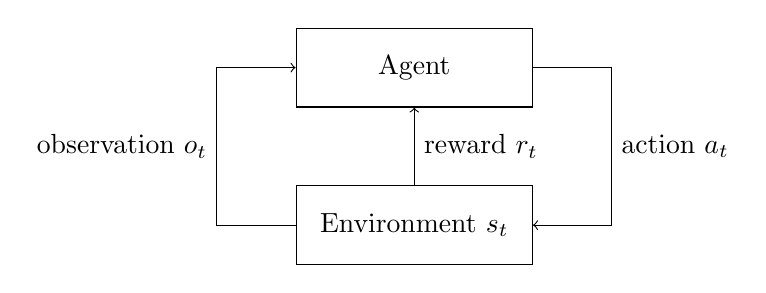
\begin{tikzpicture}[node distance=2cm]
    \tikzstyle{block} = [rectangle,minimum width=3cm,minimum height=1cm,text centered,draw=black,fill=white]
    \node (agent)[block]{Agent};
    \node (environment)[block,below of=agent]{Environment \(s_t\)};
    \draw [->] (agent.east) -- ++(1cm,0) -- node [anchor=west]{action \(a_t\)} ++(0,-2cm) -- (environment.east);
    \draw [->] (environment.north) -- node [anchor=west]{reward \(r_t\)} (agent.south);
    \draw [->] (environment.west) -- ++(-1cm,0) -- node [anchor=east]{observation \(o_t\)} ++(0,+2cm) -- (agent.west);
\end{tikzpicture}
    \label{fig:pomdp}
    \caption[Partially observable Markov decision process]{Partially observable Markov decision process.}
\end{figure}

The agent and environment interact over a sequence of discrete time steps \(t = 0, 1, \dots, T\), giving rise to an \textit{episode} of length \(T\).
At each time step \(t\), the goal of the agent is to select the action that maximizes the expected \textit{discounted return}:

\[ 
    \mathbb{E} \left[ \sum_{k=0}^T \gamma^{k-t-1} r_k \right]
\]

Since the agent receives partial observations of the environment's state, it has to act under uncertainty.
Planning in a POMDP is undecidable, and solving them is often computationally intractable.
Approximate solutions are more common, where the agent usually maintains an internal \textit{belief state}~\cite{kaelbling_pomdp_1998} which is acts on.
The belief state summarizes the agent's previous experience and is therefore dependent on the full \textit{history} of actions and observations.
It does not need to summarize the whole history, but generally only the information that helps the agent maximize the expected reward.
From here on we will use the belief state and the environment state \(s\) interchangably. 
% Sutton page 467 is better, contains latent state assumption


\subsubsection{Policies and Value Functions}
\label{sec:policy-value}

The behaviour of the agent is described by its \textit{policy}.
A policy \(\pi\) is a mapping from perceived environment states to actions.
Policies are often stochastic and specify probabilities for each action, with \(\pi(a|s)\) denoting the probability of taking action \(a\) in state \(s\).~\cite{sutton_reinforcement_2018}

Most RL solutions methods also approximate a \textit{value function}.
A value function \(v_\pi\) estimates how good it is to be in a state.
The value function \(v_\pi(s)\) is the expected (discounted) return when starting at state \(s\) and following policy \(\pi\) until the end of the episode.
There are two common alternative value functions:
The \textit{quality function} \(q_\pi(s,a)\) gives the value of state \(s\) under policy \(\pi\) where \(a\) is the first action taken.
Given a quality function, \textit{action-value} methods choose the action greedily at every state as \(arg\,max q_\pi(s, a)\).
The \textit{advantage function} \(a_\pi(s, a)\) instead represents the relative advantage of actions, \(a_\pi = q_\pi - v_\pi\).~\cite{sutton_reinforcement_2018}

For problems with large state and action spaces, it is common to represent value functions with \textit{function approximation}.
In such cases, it is common to encounter states that have never been encountered before.
This makes it important that the estimated value function can generalize from seen to unseen states.
With examples from the true value function, an approximation can be made with supervised learning methods.
We write \(\hat{v}(s,\mathbf{w}) \approx v_\pi(s)\) for the approximate value of state \(s\) with some weight vector \(\mathbf{w} \in \mathbb{R}^d\).~\cite{sutton_reinforcement_2018}

An alternative to action-value methods is to approximate the policy itself.
\textit{Policy gradient methods}~\cite{sutton_policygrad_1999} learn a parametrized policy that select actions without a value function.
We denote a parametrized policy as \(\pi(a|s,\boldsymbol{\theta})\) with \(\boldsymbol{\theta} \in \mathbb{R}^{d^\prime}\) as the parameters to the policy.
The policy parameters are usually learned based on the gradient of some performance measure \(J(\boldsymbol{\theta})\).
As long as \(\pi(a|s,\boldsymbol{\theta})\) is differentiable with respect to its parameters, the parameters can be updated with \textit{gradient ascent} in \(J\):

\[
    \boldsymbol{\theta}_{t+1} = \boldsymbol{\theta}_t + \alpha \hat{\nabla J(\boldsymbol{\theta}_t)}) 
\]

Advantages of policy parametrization over action-value methods include stronger convergence guarantees~\cite{sutton_policygrad_1999} and more flexibility in parametrization~\cite{sutton_reinforcement_2018}. In practice, value functions are often still used to learn the policy parameter, but they are not needed for action selection.
Such methods are called \textit{actor-critic} methods, with actor referring to the learned policy and critic referring to the learned value function.
In these cases, there might also be some overlap between the weights \(\mathbf{w}\) of the value function estimate and \(\boldsymbol{\theta}\) of the policy estimate. 

Function approximation includes important aspects of partial observability.
If there is a state variable that is not observable,
then the parametrization can be chosen such that the approximate value does not depend on that state variable.
Because of this, function approximation is applicable to the partially observable case.

% https://www.quora.com/What-are-the-benefits-of-actor-critic-framework-in-reinforcement-learning

% We might imagine an artificial neural network (ANN) in which the last layer is split into multiple parts, or heads, each working on a di↵erent task. One head might produce the approximate value function for the main task (with reward as its cumulant) whereas the others would produce solutions to various auxiliary tasks. All heads could propagate errors by stochastic gradient descent into the same body—the shared preceding part of the network—which would then try to form representations, in its next-to-last layer, to support all the heads. Researchers have experimented with auxiliary tasks such as predicting change in pixels, predicting the next time step’s reward, and predicting the distribution of the return. In many cases this approach has been shown to greatly accelerate learning on the main task (Jaderberg et al., 2017). Multiple predictions have similarly been repeatedly proposed as a way of directing the construction of state estimates (see Section 17.3). (Sutton)

\subsubsection{Challenges in Reinforcement Learning}

% we can illustrate the challenges in terms of our problem

One of the challenges that arises in reinforcement learning is the exploration-exploitation trade-off.
An RL agent should \textit{exploit} knowledge gained from previous experiences and prefer actions that has yielded reward in the past.
It should also \textit{explore} in order to learn better actions to take in the future.
Agents that fail to both exploit and explore will lead to failure at the task.
%Furthermore, striking a good balance between the two is non-trivial, and often requires care.~\cite{sutton}

Another challenge is the design of reeward signals.
For some tasks, like certain video games, the objective is simply to maximize the score obtained.
In this case there is an inherent reward signal and the agent achieves its task simply by maximizing this inherent signal.
Other times, we have a task we want the agent to solve and have to design a reward signal around that task.
Designing rewards is not straight-forward and can often have unintended effects~\cite{sutton_reinforcement_2018}.
Special care has to be taken to ensure that the reward incentivizes the desired behaviour.

Here, the problem of \textit{sparse rewards} also comes into play.
The agent has to be reward frequently enough to allow it to achieve its goal once.
Often it has to incentivize it to achieve its goal efficiently, with multiple different starting conditions.
If rewards are too sparse, the agent may explore aimlessly and take too long to find achieve its goal.
In such cases, it can be effective to modify the reward to give the agent hints along the way.
If the received reward is temporally distant from the action that caused it, the agent may have difficulty connecting the two.
This is known as the \textit{credit assignment problem}~\cite{minsky_cap_1961}.

In practice, rewards are often designed through trial-and-error.
Several iterations of a reward signal are tried until one yields expected and sufficient results.

% Reward shaping is a technique to tackle\dots~\cite{mataric_shaping_1994}
% https://ai.stackexchange.com/questions/12908/what-is-the-credit-assignment-problem
% https://medium.com/@m.k.daaboul/dealing-with-sparse-reward-environments-38c0489c844d
% reward shaping

\subsection{Deep Learning}

Deep learning is a family of techniques in which hypothesis are represented as computation graphs with tunable weights.
The computation graphs are inspired by biological neurons in the brain and are referred to as \textit{neural networks}.
Deep neural networks consist of \textit{nodes} arranged in \textit{layers}: one input layer, zero or more hidden layers and one output layer.
Each layer receives an input \textit{representation}~\cite{bengio_representation_2014} from the previous layer and outputs a transformed representation to the next layer.
Given some input, a neural network optimizes its output representation with regard to some criterion.
Usually, a loss function \(\mathcal{L}\) is minimized by updating the weights \(\mathbf{w}\) of the network with some variant of \textit{gradient descent} with learning rate \(\alpha\):

\begin{equation}
    \mathbf{w} \leftarrow \mathbf{w} - \alpha \nabla_\mathbf{w} \mathcal{L}(\mathbf{w}) 
\end{equation}

The only requirement on the functions computed by each node is that it is differentiable.
As long as this holds, layers can be stacked arbitrarily and the gradients can be computed with the chain rule.
This way, errors in the output can be passed back through the network (\textit{back-propagation}) and used to update the weights.~\cite{russell_artificial_2021,goodfellow_deep_2016}

The architecture of a neural network imposes some bias onto the learning that its expected to be useful for generalizing to unseen samples.
We now describe three neural network architectures that will be used in this work.

\subsubsection{Feedforward Neural Network}

A feedforward neural network, also known as a multi-layer perceptron (MLP)~\cite{goodfellow_deep_2016}, only has connections in one direction.
Each node in the network receives inputs from its predecessors and outputs the result of a function of those inputs.
The output \(y\) of each node is usually computed by taking the weighted sum of its inputs \(x\) and applying some non-linear function

\begin{equation}
    y_j = g_j(\mathbf{w}_j^T \mathbf{x}),
\end{equation}

where \(y_j\) is the output of node \(j\), \(g_j\) is a non-linear \textit{activation function}, \(\mathbf{w}_j\) is the vector of weights leading into node \(j\), and \(\mathbf{x}\) is the vector of inputs to the node.
By convention, each layer also has some \textit{bias} that allows the total weighted input to \(g_j\) to be non-zero even when the outputs from the previous layer are zero.
The bias is included as an extra input \(x_0\) fixed to 1, and an extra tunable weight \(w_{0,j}\).
The non-linearity ensures that a network with at least two layers can approximate any continuous function.~\cite{russell_artificial_2021}

\subsubsection{Convolutional Neural Network}

Convolutional Neural Networks (CNNs) contain spatially local connections.
They have patterns of weights, called \textit{kernels}, that are replicated across units in each layer.
With some input vector \(\mathbf{x}\) of size \(n\) and a vector kernel \(\mathbf{k}\) of size \(l\), the (discrete) convolution operation \(\mathbf{z} = \mathbf{x} \ast \mathbf{k}\) is defined as

\begin{equation}
    z_i = \sum_{j=1}^l k_j x_{j+1-\frac{l+1}{s}},
\end{equation}

where \(s\) is the \textit{stride}.
This operations can be generalized up to more than one dimension, such as 2 dimensions for images and 3 dimensions for volumes.
With multiple input channels, kernels are stacked into a \textit{filter}.
The outputs of each kernel are then summed over, giving one output channel per filter.

There are several advantages to using CNNs for structured input data where neighboring values are correlated.
Kernels are smaller than the input, which means that fewer parameters have to be stored.
These \textit{sparse interactions} give CNNs reduced memory requirements,
as well as improved statistical and computational efficiency.

Furthermore, the same parameters are also used for more than one function in the CNN. \textit{Parameter sharing} across input locations mean that layers in a CNN have \textit{equivariance} to translation. 
The output of one kernel is the same regardless of the input location.
This property of CNNs is useful for images where similar features may be useful regardless of their location in the input.~\cite{goodfellow_deep_2016}

%A common augmentation to deep CNNs is \textit{residual networks}.

\subsubsection{Recurrent Neural Network}

Recurrent neural networks (RNNs) extend feedforward networks by allowing cycles in the computation graph.
Each cycle has a delay so that some \textit{hidden state} from the previous computation is used as input to the current computation.
A recurrent layer with input \(\mathbf{x}_t\), output \(\mathbf{y}_t\) and hidden state \(\mathbf{z}_t\) is defined by

\begin{align}
    \begin{split}
        \mathbf{z}_t &= f_\mathbf{w}(\mathbf{z}_{t-1}, \mathbf{x}_t) \\
        \mathbf{y}_t &= g_y(\mathbf{W}_{z,y}, \mathbf{z}_t),
    \end{split}
\end{align}

where \(f_\mathbf{w}\) is the update process for the hidden state and \(g_y\) is the activation function for the hidden layer.
This model can be turned into a feedforward network over a sequence of input vectors \(\mathbf{x}_1, \dots \mathbf{x}_T\) and observed outputs \(\mathbf{y}_1, \dots, \mathbf{y}_T\) by \textit{unrolling} it for \(T\) steps. The weights are shared across all time steps. This means that RNNs can operate on inputs of arbitrary lengths.
The hidden state is used as a summary of all previous items in the sequence.
Thus, RNNs make a Markov assumption.~\cite{russell_artificial_2021}

In practice, conventional RNNs struggle with learning long-term dependencies.
During back-propagation, gradients can tend to zero for long sequences, something known as the vanishing gradient problem~\cite{goodfellow_deep_2016}.
An architecture that addresses this issue is long short-term memory (LSTM)~\cite{hochreiter_schmidhuber_lstm_1997}.
LSTMs include a \textit{memory cell} \(c\) in the hidden state that is copied from time step to time step, and three soft \textit{gating units} that govern the information flow in the hidden state update process \(f\). This makes LSTMs particularly useful for learning over long sequences.

\section{Related Work}

To our knowledge, there is no work that considers the exact problem we are looking at.
In this section, we present work that considers similar tasks.

\subsection{Deep Reinforcement Learning}

% Mnih et al., Atari, DQN

As mentioned in Section~\ref{sec:policy-value}, policies and value functions are often approximated.
Neural networks have good properties for function approximation and have been used for RL with success.
One early example is TD-Gammon~\cite{tesauro1995tdgammon}, a neural network trained with RL that reached expert Backgammon performance in 1995.

More recently, the successes of deep learning have bled over into the field of RL.
In 2015, Mnih et al.~\cite{mnih_human_2015} extend \cite{mnih_atari_2013} and introduce DQN, which combines deep neural networks with RL and gives birth to the field of deep reinforcement learning (deep RL).
DQN approximates the quality function \(q(s, a)\) with a CNN, and select actions greedily using only visual input.
To incorporate some memory, images from the 4 previous time steps are stacked and used as input to the neural network.
The input is fed through three convolutional layers:
32 \(8\times8\) filters with stride 4,
followed by 64 \(4\times4\) filters with stride 2,
followed by 64 filters of size \(32\times32\) with stride 1.
Between each convolutional layer is a ReLU activation function.
Then, there is a hidden fully connected layer with a ReLU activation function.
The output layer has one output for each valid action.
% replay buffer
% instability
% follow up works
% architecture
%\cite{arulkumaran_survey_2017}

The DQN architecture sparked great interest and several modifications.
Hausknecht and Stone (2017)~\cite{hausknecht_stone_2017} investigate the effects of adding a recurrent step to DQN in order to tackle POMDPs.
They use the same convolutional network as \cite{mnih_human_2015}, but only use the most recent frame as input and replace the hidden layer with a recurrent LSTM.
It is found that the agent is able to integrate information over time and achieves comparable performance to the original DQN agent.

\subsection{Proximal Policy Optimization}

Proximal policy optimization algorithms\dots~\cite{schulman_ppo_2017}.

\begin{algorithm}
    \caption{Proximal Policy Optimization}
    \begin{algorithmic}
        \For{\(\text{iteration} = 1,2,\dots\)}
            \For{\(\text{actor} = 1,2,\dots,N\)}
                \State \(\text{Run policy } \pi_{\theta_\text{old}} \text{ for } T \text{ timesteps}\)
                \State \(\text{Compute advantage estimates } \hat{A}_1, \dots \hat{A}_T\)
            \EndFor
            \State \(\text{Optimize surrogate } L \text{ wrt } \theta, \text{ with } K \text{ epochs and minibatch size } M \leq NT\)
            \State \(\theta_{\text{old}} \leftarrow \theta\)
        \EndFor
    \end{algorithmic}
\end{algorithm}

\subsection{Object Detection}

% active object detection

In computer vision, \textit{object detection} is the task of detecting semantic objects of a certain class in images.
Detecting an object entails \textit{recognizing} that it is present in an image, and \textit{localizing} it by determining its bounding box.
State of the art object detection uses deep learning techniques and usually involves a CNN~\cite{zhao_objectdetection_2019}.

Although we do not focus on difficult recognition problems in this work, the task we consider bears resemblance to object localization.
Object detectors usually use region proposal networks that consider the whole image and return a set of bounding box candidates.
The object recognizer is then run on each region proposal.


Usually, images in object detection are passively sampled - they are drawn from some distribution and all are independent.
In \textit{active object detection}, images are instead chosen so as to 


Caicedo and Lazebnik~\cite{caicedo_active_2015} propose to use deep reinforcement learning for active object localization in images where the object to be localized is fully visible.
An agent is trained to successively improve a bounding box using translating and scaling transformations.
They use a reward signal that is proportional to how well the current box covers the target object.
An action that improves the region is rewarded with +1, and given a punishment of -1 otherwise.
They find that this reward communicates more clearly which transformations keep the object inside the box and which take the box away from the target.
When there is no action that improves the bounding box, the agent may select a trigger action (which would be the only action that does not give a negative reward) which resets the box.
This way the agent may select additional bounding boxes.
Each trigger modifies the environment by marking it so that the agent may learn to not select the same region twice. % inhibition-of-return mechanism, widely used in visual attention models ~\cite{itti_koch_2001}




A similar work by Ghesu et al.~\cite{ghesu_artificial_2016} present an agent for anatomical landmark detection trained with DRL.
Different from \cite{caicedo_active_2015} is that the entire scene is not visible at once.
The agent sees a limited region of interest in an image, with its center representing the current position of the agent.
The actions available to the agent translate the view up, down, left and right.
A reward is given to the agent that is equal to the supervised relative distance-change to the landmark after each action.
Three datasets of 891 anatomical images are used.
The agent starts at random positions in the image close to the target landmark and is tasked with moving to the target location.
While achieving strong results (90\% success rate), the scenes and targets are all drawn from a distribution with low variance.
Most real-world search tasks exhibit larger variance than anatomical images of the human body.


% not that relevant now that I read it
% Uzkent et al.~\cite{uzkent_detection_2020} use deep RL to detect obects in large images.
% A policy network is trained to select between high and low level of detail in images in order to reduce the computational requirements.
% http://xviewdataset.org/ is used by Uzkent - looks promising

% CT scan material: there is way less variance, otherwise similar. Big difference is that we look at more variance in many aspects?
% CV material: different in that the object is assumed to be visible

Chen and Gupta~\cite{chen_memory_2017} use a spatial memory for context reasoning in object detection\dots

\subsection{Visual Attention}

Visual attention in humans is often split into two phasesis usually split into two phases

~\cite{itti_koch_2001}


% this article is very good!
% note: reinforcement learning part, soft and hard attention
% https://shairozsohail.medium.com/a-survey-of-visual-attention-mechanisms-in-deep-learning-1043eb25f343

% "Looking through a foggy pane of glass represents soft attention, where the entire image is still being “seen”, but certain areas are being attended to more. Whereas the binoculars represent hard attention, where we are only seeing a subset of the image, hopefully the part most relevant to our task. The Recurrent Models of Visual Attention paper from above represents hard attention. The key thing to take away is that there are explicit trade-offs between these attention types: hard attention requires significantly less computation and memory (as the entire image is not being stored or operated over usually) but cannot be easily trained as the objective is non-differentiable (there is no gradient, pixels are either seen or unseen). Hence it is often trained with methods like REINFORCE. Soft attention on the other hand often requires more memory and computation (often even more then simple convolutional nets) but has a differentiable objective and can be easily trained with standard back propagation methods." <- some good points here

% closely connected with object detection

\cite{minut_mahadevan_2001}

\cite{mnih_attention_2014}

Soft attention (Bahdanau~\cite{bahdanau_attention_2016})\dots

Partially observable processes, such as the one we consider in this work, can be seens as hard attention problems.
By taking actions, the hard attention can be redirected.


\subsection{Coverage Path Planning}

% could be a smaller section in background, under visual search

The problem we consider in this work shares many characteristics with coverage path planning (CPP)~\cite{galceran_carreras_2013}.
CPP is the task of determining a path that passes over all points in an area, and appears as a fundamental part of many real-world problems. 
In the general case, an agent that does not learn to exhaustively search its environment can not be expected to be successful for the visual search task.
The CPP is strongly related to the traveling salesman problem (TSP).
The unrestricted CPP where there are no obstacles (the "lawnmower problem") is in fact proven to be NP-hard~\cite{arkin_lawnmowing_2000}.
In our problem, we do not require complete coverage, but just that certain points (those that contain targets) are visited.
The shape of the environment is known, as the sensor has limited range of movement.
Furthermore, a good agent should also prioritize certain regions which is not part of the CPP task.
Although a CPP agent that is able to recognize targets is not optimal, it is a suitable baseline for the task.
Specifically, the wavefront algorithm~\cite{galceran_carreras_2013} which is suitable for grid-discretized can be used. % some simple approximation

% \cite{krishna_tetromino_2020} -connection to RL

\subsection{Visual Navigation}

The task we consider bears resemblance to visual navigation~\cite{zeng_survey_2020}. % or is an instance of?

% Point navigation / Object Navigation




Mnih et al. (2016)~\cite{mnih_asynchronous_2016} use a recurrent policy with only RGB images to navigate in a labyrinth.
3D labyrinths are randomly generated, and an agent is tasked with finding objects in them.
The same architecture as in \cite{mnih_human_2015} is used, but with 256 LSTM cells after the final hidden layer.

% https://aihabitat.org/challenge/2020/#task-1-pointnav
% https://aihabitat.org/challenge/2020/#task-2-objectnav
% https://arxiv.org/pdf/1709.06158.pdf
% https://ieeexplore.ieee.org/document/9102361


Mirowski et al. (2017)~\cite{mirowski_navigate_2017}...

Henriques and Vedaldi (2018)~\cite{henriques_vedaldi_2018} use a spatial memory...

Gupta et al. (2019)~\cite{gupta_cognitive_2019} use a latent spatial memory.
The 
They also use a planner that can plan paths given partial information of the environment.
This allows the agent to take appearance of visited locations into account when deciding where to look next.
The RGB observation is fed through an encoder network that\dots
Planning in this fashion s
% has a list of baselines
% among them is an lstm baseline

Dhiman et al. (2019)~\cite{dhiman_critical_2019} critically investigate deep RL for navigation.
They ask whether DRL algorithms are inherently able to gather and exploit environmental information for during navigation.
Experimentally, they find that an agent is able to exploit environment information when trained and tested on the same map.
However, when trained and tested on differen maps, it cannot do so succesfully.
They further find that, with a single decision point whose correct\dots
% could be due to their inductive biases
% the agent does not have access to its location and can therefore not determine its location
% their setup:
% - random maze
% - when agent finds goal, it respawns and the goal is at the same location (+10)
% - smaller rewards scattered in area to incentivize exploration (+1)
% - wall penalty (-2)
% - respawn either static or random
% - randomly textured walls

Chaplot et al. (2020)~\cite{chaplot_semantic_2020} build on the idea of an explicit memory by including environment semantics\dots

Zhu et al. (2016)~\cite{zhu_target_driven_2016} create a model for target-driven visual navigation in indooor scenes with DRL.
An observer is given a partial image of its scene as well as an image of the target object, and is tasked with navigating to the object n the scene with a minimal number of steps.
The agent moves forwards, backwards, and turns left and right at constant step lengths.
They use a reward signal with a small time penalty to incentivize task completion in few steps.
They compare their approach to random walk and the shortest path and achieve promising results.
This setup is quite similar to the one considered in this report, but the authors make a few assumptions that we do not.
They a set of 32 scenes, each of which contain a fixed number of object instances.
They focus on learning spatial relationships between objects in these specific scenes, and have scene-specific layers to achieve this.
Thus, while they show that they can adapt a trained network to a new scene, their approach is unable to zero-shot generalize to new scenes.

A similar work by Ye et al. (2018)~\cite{ye_active_2018} integrates an object recognition module with a deep reinforcement learning based visual navigation module.
They experiment with a set of reward functions and find that constant time penalizing rewards can be problematic and lead to slow convergence.
Their experiments make the same assumptions as \cite{zhu_target_driven} - the scenes and targets used during testing have all been seen during training.

Several works in visual navigation have placed emphasis on memory representations.~\cite{savinov_topmem_2018,oh_minecraft_2016,parisotto_salakhutdinov_2017,chen_memory_2017} % cite more

\subsection{Memory Architectures for Deep Reinforcement Learning}

\begin{enumerate}
    \item Frame stacking
    \item Recurrent networks
    \item Explicit memories~\cite{oh_minecraft_2016,parisotto_salakhutdinov_2017}.
    % oh remembers over the past K frames, parisotto remembers the entire world
    % parisotto tests on 3d environment. if we don't, we should at least discuss it.
\end{enumerate}


Oh et al. ~\cite{oh_minecraft_2016} use a differentiable retrieval memory.

Parisotto and Salakhutdinov~\cite{parisotto_salakhutdinov_2017} propose a structured memory\dots % this one is very interesting

% could have a section for memory mechanisms
% this is detailed in the survey \cite{arulkumaran_survey_2017}
% Taking recurrent processing further, it is possible to add a differentiable memory to the DQN, which allows it to more flexibly process information in its “working memory” [96]. In traditional RNNs, recurrent units are responsible for both performing calculations and storing information. Differentiable memories add large matrices that are purely used for storing information, and can be accessed using differentiable read and write operations, analagously to computer memory. With their key-value-based memory Q-network (MQN), Oh et al. [96] constructed an agent that could solve a simple maze built in Minecraft, where the correct goal in each episode was indicated by a coloured block shown near the start of the maze. The MQN, and especially its more sophisticated variants, significantly outperformed both DQN and DRQN baselines, highlighting the importance of using decoupled memory storage. More recent work, where the memory was given a 2D structure in order to resemble a spatial map, hints at future research where more specialised memory structures will be developed to address specific problems, such as 2D or 3D navigation [98]. Alternatively, differentiable memories can be used as approximate hash tables, allowing DRL algorithms to store and retrieve successful experiences to facilitate rapid learning [105].


Anderson et al. (2018)~\cite{anderson_evaluation_2018} emphasize the importance of memory mechanisms that support the construction of rich internal representations environments in navigation agents.
Simple agents that are purely reactive and act on the sensory input at the current time step only work for simple tasks.
Agumentations like reucrrent update mechanisms add more potential.
More advanced memory mechanisms can be important for better navigation.
The nature of the internal representation is central to the study of embodied navigation.
% more recommendations are there, are they relevant?
% see citations [12, 13, 22, 23, 27] on memory mechanisms
% \cite{gupta_cognitive_2019}
% 


\subsection{Benchmarking Environments}

\begin{itemize}
    \item What is contained in an environment (represents a Markov Decision Process).
    \item What is a good benchmarking environment
    \item Should list some common environments and explain why they are not satistfactory
\end{itemize}

\subsection{Inductive Biases, Overfitting and Generalization in Deep Reinforcement Learning}

% first introduce the reason why generalization is important
% reality is dynamic
% agents need to be robust to variation
% capability to transfer and adapt to unseen but similar environments
% most current research works on benchmarks that do not test this (MuJoCo, Arcade learning environment)

Kirk et al. (2021)~\cite{kirk_survey_2022} survey generalization in deep RL.

% refer to survey
% specifically IID (train_dist = test_dist) and OOD environments (train_dist != test_dist)

While deep neural networks have proved to be effective function approximators for RL, they are also prone to \textit{overfitting}.
High-capacity models trained over a long time may memorize the distribution seen during training rather than general patterns.
While studied in supervised learning, overfitting is generally been neglected in deep RL.
Training and evaluation stages are typically not separated.
Instead, the final return on the training environments is used as a measure of agent performance.

Zhang et al. (2018)~\cite{zhang_overfitting_2018} study overfitting and generalization in deep RL.
With experiments, they show that RL agents are capable of memorizing training data, even when completely random.
When the number of training samples exceeds the capacity of the agent, they overfit to them.
When exposed to new but statistically similar environments during testing, test performance could vary significantly despite consistent training performance.
The authors argue that good generalization requires that the \textit{inductive bias} of the algorithms is compatible with the bias of the problems.
The inductive bias refers to a priori algorithmic preferences, like neural network architecture.
When comparing MLPs with CNNs, they find that MLPs tend to be better at fitting the training data are worse at generalizing.
When rewards are spatially invariant, CNNs generalize much better than MLPs.
The authors advocate for carefully designed testing protocols for detecting overfitting.
The effectiveness of stochastic-based evaluation depends on the properties of the task.
Agents could still learn to overfit to random training data. 
For this reason, they recommend isolation of statistically tied training and test sets.

In a similar spirit, Cobbe et al. (2019)~\cite{cobbe_generalization_2019} construct distinct training and test sets to measure generalization in RL.
They find that agents can overfit to surprisingly large training sets, and that deep convolutional architectures can improve generalization.
Methods from supervised learning, like L2 regularization, dropout, data augmentation and batch normalization are also shown to aid with generalization.

Many current deep RL agents do not optimize the true objective that they are evaluated against,
but rather a handcrafted objective that incorporates biases to simplify learning.
Stronger biases can lead to faster learning, while weaker biases potentially lead to more general agents.
Hessel et al. (2019)~\cite{hessel_inductive_2019} investigate the trade-off between generality and performance from the perspective of inductive biases.
Through experimentation with common reward sculpting techniques, they find that learned solutions are competitive with domain heuristics like handcrafted objectives.
Learned solutions also seem to be better at generalizing to unseen domains.
For this reason, they argue for removing biases determined with domain knowledge in future research.


% what does this mean for "oracle" reward signals, such as supervised improvement in distance? 
% it is essentially reward shaping.
% they introduce human bias into the possible policies.
% the agent may fail to discover optimal policies.
% the problem with our reward is that I am not sure it will lead to minimizing time.
% should run experiments with time penalty and trigger reward again...

% in this spirit
Cobbe et al. (2020)~\cite{cobbe_procgen_2020} introduce a benchmark for sample efficiency and generalization in RL.
They make use of procedural generalization to decide many parameters of the initial state of the environment.
This forces agents to learn policies that are robust variation and avoid overfitting.
To evaluate sample efficiency of agents in the benchmark, they train and test on the full distribution of states.
To evaluate generalization, they fix the number of training samples and then test on held out levels.
When an episode ends, a new sample is drawn from the training set.
Agents may train for arbitrarily many time steps.
The number of training samples required to generalize is dependent on the particulars and difficulty of the environment.
The authors choose the training set size to be near the region when generalization begins to take effect.
Empirically they find that larger model architectures improve both sample efficiency and generalization.
Agents strongly overfit to small training sets and need many samples to generalize.
Interestingly, training performance improves as the training set grows past a certain threshold.
The authors attribute this to the implicit curriculum of the distribution of levels.

\subsection{Evaluation of Deep Reinforcement Learning Agents}

A problem in state-of-the art RL is reproducibility.
There is often non-determinism, both in the methods and environments used.
Furthermore, many methods have intrincic variance which can make published results difficult to interpret.
This has meant that reproducing state-of-the-art deep RL results is difficult.

Henderson et al.~\cite{henderson_matters_2018} discuss this problem from multiple perspectives.
Through experimental analysis, they show that:

\begin{itemize}
    \item In policy gradient methods, hyperparameters and the choice of network architecture for policy and value function approximation can affect performance significantly.
    They find that ReLU activations tend to perform best across environments and algorithms.
    For PPO, the use of large networks may require changing other hyperparameters like learning rate.
    \item Rescaling rewards can have a large effect, although it is difficult to predict how.
    \item Variance between random seeds in stochastic environments affects performance of algorithms, and give learning curves that do not fall within the same distribution.
    This suggests that selecting the top \(N\) trials or average over a small number of trials \(N\) can be misleading. They suggest to compare performance over many different random seeds.
    \item For certain environments, learning curves can indicate successful optimization but the learned behaviour may not be satisfactory.
    It is therefore important to not only show returns, but also demonstrations of the learned policy in action.
    \item Implementation differences that are not reflected in publications can have a dramatic impact on performance.
    It is therefore necessary to enumerate implementation details and package codebases with publications.
    Performance of baseline experiments should also match original baseline publication code.
\end{itemize}

Due to the unstable nature of RL algorithms, it is often inadequate to just report average return.
\cite{henderson_matters_2018} propose to include confidence intervals when reporting results.
Confidence bounds with sample bootstrapping is used to show that PPO is among the more stable algorithms.
Various other significance tests\dots

Finally, \cite{henderson_matters_2018} make the point that more emphasis should be placed on applying RL algorithms to real-world tasks.
Benchmarks environments like ALE~\cite{arcade} often have no clear winner.
It could be more useful to propose a set of tasks that an algorithm could be used for than to show performance on fictional tasks.

A similar work by Agarwal et al. (2022)~\cite{agarwal_rlliable_2022} criticises the heavy use of point estimates of aggregate performance.
They show that conclusions drawn from point estimates can be very different from those drawn from more thorough statistical analysis. 
The popularity of more challenging benchmarks has lead to longer training times.
This has made it less feasible to measure performance over many training runs,
which in turn has led to a shift to only evaluating a small number of runs per task.
Like \cite{henderson_matters_2018}, they advocate for the use  of performance metrics that take uncertainty in results into account.
They propose the following set of metrics that better reflect performance across a handful of runs:

\begin{itemize}
    \item Uncertainty in aggregate performance should be reported through interval estimates via stratified bootstrap confidence intervals.
    \item Variability in performance across tasks should be reported through performance profiles (score distributions).
    \item Aggregate metrics for summarizing performance across tasks should be reported through interquartile mean (IQM) across all runs.
\end{itemize}

Anderson et al. (2018)~\cite{anderson_evaluation_2018} discuss problem statements and evaluation measures for embodied navigation agents, and make a set of recommendations.
A navigation agent should be equipped with a special action that indicates that it has concluded the episode.
The agent should be evaluated at the time this action is made, and not at some more favorable time step. % implicitly the trigger action for us, since we have multiple targets
Proximity to a goal should be measured using geodesic distance, the shortest distance in the environment. % Manhattan in 2D?
They recommend success weighted by (normalized inverse) path length (SPL) as the primary measure of navigation performance.
With \(N\) test episodes, SPL is computed as 

\begin{equation}
    \frac{1}{N} \sum_{i=1}^N S_i \frac{l_i}{\max(p_i, l_i)}
\end{equation}

% if we adopt SPL, we should note that the optimal path is not realistic for this problem

where \(S_i\) is a binary indicator of success,
\(l_i\) is the shortest path distance from the agent's starting position to the goal,
and \(p_i\) is the length of the path actually taken in the episode.
If 50\% of test episode are successful and the agent takes the optimal path in all of them, its SPL is 0.5.
By measuring SPL of human subjects, what is a good score can be calibrated.

Batra et al. (2020)~\cite{batra_evaluation_2020} revisit the problem of evaluating embodied navigation agents.
They note some issues with the SPL metric.
It fails to consider the fact that some failures are less of a failure than others.
Some failures might in fact be close to reaching the goal while some fail completely.
The binary success introduces high variance in average SPL computation.
Furthermore, SPL is not particularly suitable for comparison across different datasets,
as obtaining a high SPL is more difficult for short paths than for long paths.
They suggest that SPL should be replaced by some metric that takes these issues into account.
However, to our knowledge such a metric is yet to be proposed and widely adopted.